%-------------------------
% Resume in Latex
% Author : Jake Gutierrez
% Based off of: https://github.com/sb2nov/resume
% License : MIT
%------------------------

%\documentclass[letterpaper,11pt]{article}
\documentclass[a4paper,10pt]{article}

\usepackage{latexsym}
\usepackage[empty]{fullpage}
\usepackage{titlesec}
\usepackage{marvosym}
\usepackage[usenames,dvipsnames]{color}
\usepackage{verbatim}
\usepackage{enumitem}
\usepackage[hidelinks]{hyperref}
\usepackage{fancyhdr}
\usepackage[english, russian]{babel}
\usepackage{tabularx}
\usepackage{graphicx}
\input{glyphtounicode}


\pagestyle{fancy}
\fancyhf{} % clear all header and footer fields
\fancyfoot{}
\renewcommand{\headrulewidth}{0pt}
\renewcommand{\footrulewidth}{0pt}

% Adjust margins
\addtolength{\oddsidemargin}{-0.5in}
\addtolength{\evensidemargin}{-0.5in}
\addtolength{\textwidth}{1in}
\addtolength{\topmargin}{-.5in}
\addtolength{\textheight}{1.0in}

\urlstyle{same}

\raggedbottom
\raggedright
\setlength{\tabcolsep}{0in}

% Sections formatting
\titleformat{\section}{
  \vspace{-4pt}\scshape\raggedright\large
}{}{0em}{}[\color{black}\titlerule \vspace{-5pt}]

% Ensure that generate pdf is machine readable/ATS parsable
\pdfgentounicode=1

%-------------------------
% Custom commands
\newcommand{\resumeItem}[1]{
  \item\small{
    {#1 \vspace{-2pt}}
  }
}

\newcommand{\resumeSubheading}[4]{
  \vspace{-2pt}\item
    \begin{tabular*}{0.97\textwidth}[t]{l@{\extracolsep{\fill}}r}
      \textbf{#1} & #2 \\
      #3 & #4 \\
    \end{tabular*}\vspace{-7pt}
}

\newcommand{\resumeSubheadingFML}[2]{
  \vspace{-2pt}\item
    \begin{tabular*}{0.97\textwidth}[t]{l@{\extracolsep{\fill}}r}
      \textbf{#1} & #2 \\
    \end{tabular*}\vspace{-7pt}
}

\newcommand{\resumeSubSubheading}[2]{
    \item
    \begin{tabular*}{0.97\textwidth}{l@{\extracolsep{\fill}}r}
      \textit{\small#1} & \textit{\small #2} \\
    \end{tabular*}\vspace{-7pt}
}

\newcommand{\resumeProjectHeading}[2]{
    \item
    \begin{tabular*}{0.97\textwidth}{l@{\extracolsep{\fill}}r}
      \small#1 & #2 \\
    \end{tabular*}\vspace{-7pt}
}

\newcommand{\resumeSubItem}[1]{\resumeItem{#1}\vspace{-4pt}}

\renewcommand\labelitemii{$\vcenter{\hbox{\tiny$\bullet$}}$}

\newcommand{\resumeSubHeadingListStart}{\begin{itemize}[leftmargin=0.15in, label={}]}
\newcommand{\resumeSubHeadingListEnd}{\end{itemize}}
\newcommand{\resumeItemListStart}{\begin{itemize}}
\newcommand{\resumeItemListEnd}{\end{itemize}\vspace{-5pt}}


%-------------------------------------------
%%%%%%  RESUME STARTS HERE  %%%%%%%%%%%%%%%%%%%%%%%%%%%%


\begin{document}

\begin{center}
    \fbox{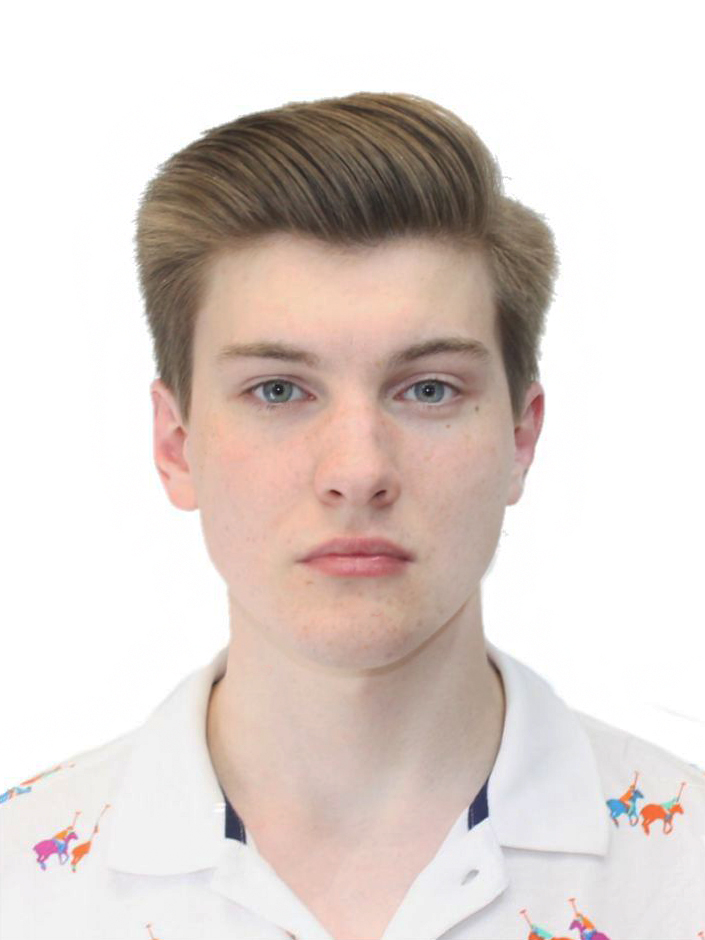
\includegraphics[scale=1]{photo.jpg}}
\end{center}

\begin{center}
    \textbf{\Huge \scshape Владислав Почернин} \\ \vspace{1pt}
    \textbf{\Large \scshape Java Junior Developer} \\ \vspace{1pt}
    \small Санкт-Петербург, Россия $|$
    \small +7-952-228-52-80 $|$ \href{mailto:vspochernin@gmail.com}{\underline{vspochernin@gmail.com}} $|$
    \href{https://t.me/vspochernin}{\underline{t.me/vspochernin}} $|$
    \href{https://github.com/vspochernin}{\underline{github.com/vspochernin}}
\end{center}


%-----------PROJECTS-----------
  \section{Опыт коммерческой разработки}
    \resumeSubHeadingListStart

      \resumeProjectHeading{\textbf{Sreda Solutions} - backend developer $|$ \emph{Java, Spring}}{Июль 2022 - Сентябрь 2022}
      \resumeItemListStart
      \resumeItem{Реализовал REST API для взаимодействия с сервисом.}
      \resumeItem{Интегрировал MockMvc в тесты контроллеров.}
      \resumeItem{Произвел рефакторинг кода в соответствии с соглашениями, принятыми на проекте.}
      \resumeItem{Создал документацию на использующиеся в проекте форматы данных.}
      \resumeItemListEnd

      \resumeProjectHeading{\textbf{Sreda Solutions} - QA $|$ \emph{Python, Appium, Allure}}{Июнь 2022 - Июль 2022}
      \resumeItemListStart
      \resumeItem{Самостоятельно изучил необходимый стек технологий для тестирования Android-приложений.}
      \resumeItem{Создал систему автоматизированного тестирования Android приложения и написал на неё документацию.}
      \resumeItem{Разработал модуль взаимодействия тестирующей программы со сторонним API.}
      \resumeItem{Разработал набор тестов, покрывающий функциональность приложения.}
      \resumeItemListEnd

      \resumeProjectHeading
	      {\href{https://github.com/PaaavelZ/FPA-pybot}{\underline{\textbf{Белорусская косметика}}} - backend developer $|$ \emph{Python, Docker, Telegram API}}{Февраль 2022 -- Май 2022}
	      \resumeItemListStart
        \resumeItem{Произвел запаковку Python-приложения в Docker-контейнер.}
        \resumeItem{Создал документацию проекта.}
	      \resumeItemListEnd

      \resumeProjectHeading
	      {\textbf{Soft-Consult} - backend developer $|$ \emph{Java, Spring Boot, PostgreSQL, Vaadin}}{Январь 2022 -- Июнь 2022}
	      \resumeItemListStart
        \resumeItem{Осуществил работу со сторонним API посредством отправки исходящих и парсинга входящих xml.}
        \resumeItem{Реализовал парсеры excel-документов и покрыл их unit тестами.}
        \resumeItem{Добавил различные компоненты UI, связав их с backend-ом.}
        \resumeItem{Произвел рефакторинг базы данных в соответствии с требованиями проекта.}
	      \resumeItemListEnd

    \resumeSubHeadingListEnd


%-----------EDUCATION-----------
\section{Образование}
  \resumeSubHeadingListStart
    \resumeSubheading
       {Политехнический Университет Петра Великого}{Санкт-Петербург, Россия}
      {Бакалавр, Программная инженерия}{Август 2020 -- Июнь 2024}

      \vspace{0.2cm}
      \resumeSubheading{Образовательный центр VK в Политехе <<Технополис>>}{Санкт-Петербург, Россия}{\href{https://polis.vk.company/curriculum/program/discipline/1611/}{\underline{Java-разработчик высоконагруженных приложений}}}{Сентябрь 2022 - Июнь 2024}

      \vspace{0.2cm}
     \resumeSubheadingFML
      {Президентский физико-математический лицей №239}{Санкт-Петербург, Россия}
  \resumeSubHeadingListEnd


%-----------PROJECTS-----------
 \section{Учебные проекты, курсы}
    \resumeSubHeadingListStart
      \resumeProjectHeading
	      {\href{https://github.com/vspochernin/architecture-2022-2023-1}{\underline{\textbf{Моделирование СМО}}} $|$ \emph{Java, Spring, Thymeleaf}}{Сентябрь 2022 -- Ноябрь 2022}
	      \resumeItemListStart
	      	\resumeItem{Разработал иммитационную модель системы массового обслуживания.}
	      	\resumeItem{Создал веб-интерфейс при помощи Spring и Thymeleaf.}
	      	\resumeItem{Произвел анализ системы, определив самые выгодные конфигурации.}
	      \resumeItemListEnd

      \resumeProjectHeading
	      {\href{https://github.com/vspochernin/java-2021-2022-1}{\underline{\textbf{СПБПУ ООП}}} $|$ \emph{Java Core, Java Multithreading, Java Concurrency}}{Сентябрь 2021 -- Январь 2022}
	      \resumeItemListStart
	      	\resumeItem{Изучил Java Core на основе курса по ООП. Был изучен основной набор технологий языка Java, включая Generics, потоки
          ввода-вывода, коллекции и многопоточное программирование.}
	      \resumeItemListEnd

      \resumeProjectHeading
	      {\textbf{Stepik} $|$ \emph{C++, Java}}{2018 -- Настоящее время}
	      \resumeItemListStart
          \resumeItem{\href{https://stepik.org/cert/1055237}{\underline{Java. Базовый курс} - Computer Science Center (CS центр)}}
          \resumeItem{\href{https://stepik.org/cert/107881}{\underline{Введение в программирование (C++)} - Академия Яндекса, Высшая школа экономики (НИУ ВШЭ)}}
	      \resumeItemListEnd

    \resumeSubHeadingListEnd

%-----------PROGRAMMING SKILLS-----------
\section{Технические навыки}
 \begin{itemize}[leftmargin=0.15in, label={}]
    \small{\item{
     \textbf{Языки}{: Java, Python, SQL, Английский B1} \\
     \textbf{Инструменты разработчика}{: Git, Docker, IntelliJ, VSCode, Linux, Vim} \\
     \textbf{Фреймворки и библиотеки}{: Spring, PostgreSQL, JUnit, Vaadin, Appium, Allure} \\
    }}
 \end{itemize}

\section{О себе}
 \begin{itemize}[leftmargin=0.15in, label={}]
    \small{\item{
    Ответственен, довожу поставленные задачи до конца. Нравится работать в команде. Люблю заниматься различными видами спорта на любительском уровне, не имею вредных привычек. В качестве хобби увлекаюсь музыкой. Постоянно совершенствую себя, изучая новое и переосмысляя старое.
    }}
 \end{itemize}

\end{document}
